\documentclass{article}

\usepackage{graphicx}
\usepackage{float}
\usepackage{caption}
\usepackage{subcaption}
\newcommand{\rulesep}{\unskip\ \vrule\ }

\begin{document}

\begin{figure}[H]
    \centering
    \captionsetup{justification=centering, size=scriptsize}
    \begin{subfigure}{0.47\textwidth}
        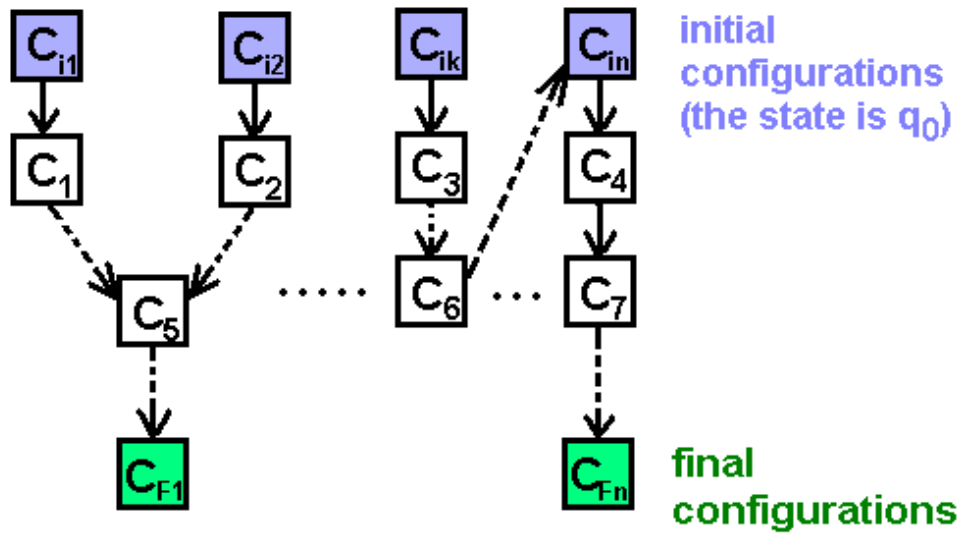
\includegraphics[width=1\textwidth, keepaspectratio]{deterministic_turing_machine_graph.png}
        \caption{Deterministic Turing machine graph}
    \end{subfigure}
    \quad
    \begin{subfigure}{0.47\textwidth}
        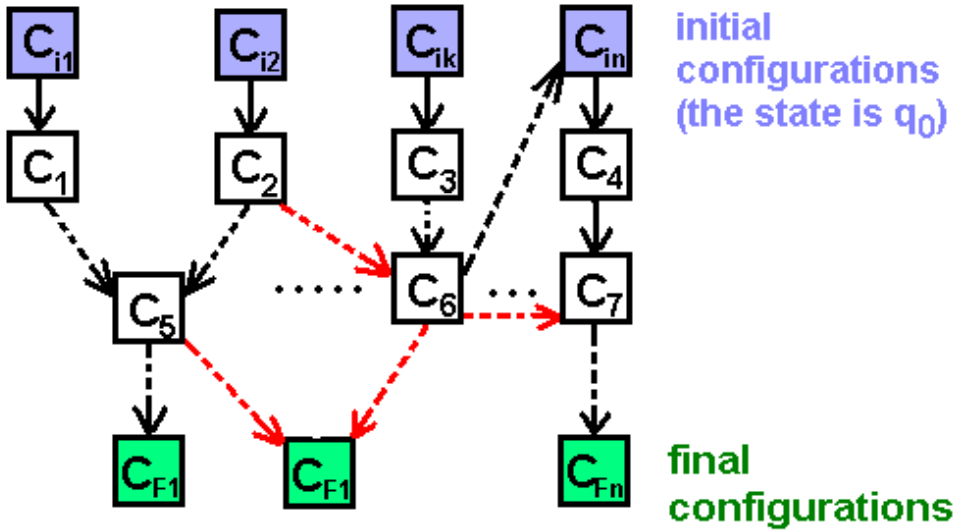
\includegraphics[width=1\textwidth, keepaspectratio]{non-deterministic_turing_machine_graph.png}
        \caption{Non-deterministic Turing machine graph}
    \end{subfigure}
    \caption{Representing Turing machines as graphs (adapted from \cite{laud_complexity_2011})}
    \label{fig:turing-machines-as-graphs}
\end{figure}

\end{document}